%!TEX root = main.tex
 \section{Evaluation Study Findings\label{sec:eval_findings}}
 % \begin{figure*}[t!]
 % \minipage{0.6\textwidth}
 %   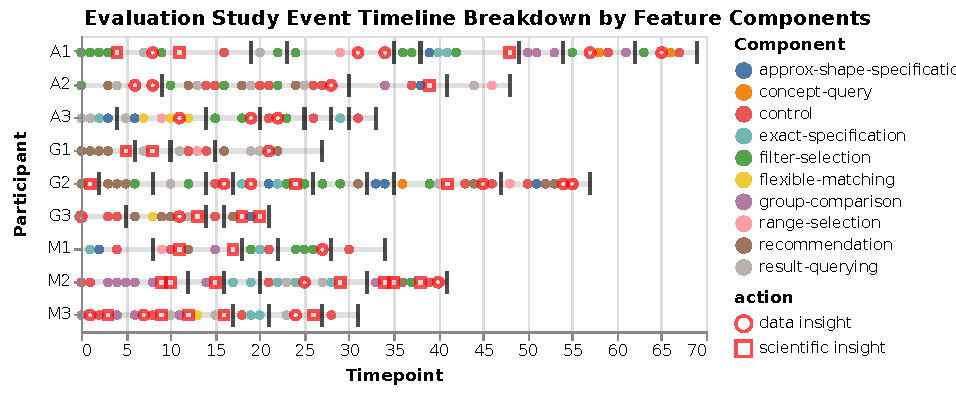
\includegraphics[width=\linewidth]{figures/evalstudytimeline.pdf}
 %   \caption{Timeline of event code and component usage, with every timepoint as an event on the x axis. For clarity, we hide most of the event coding labels other than the insight labels. Black vertical tick indicates a session break, signaling the beginning of a new line of inquiry.}\label{fig:evalstudytimeline}
 % \endminipage\hfill
 % \minipage{0.4\textwidth}
 %   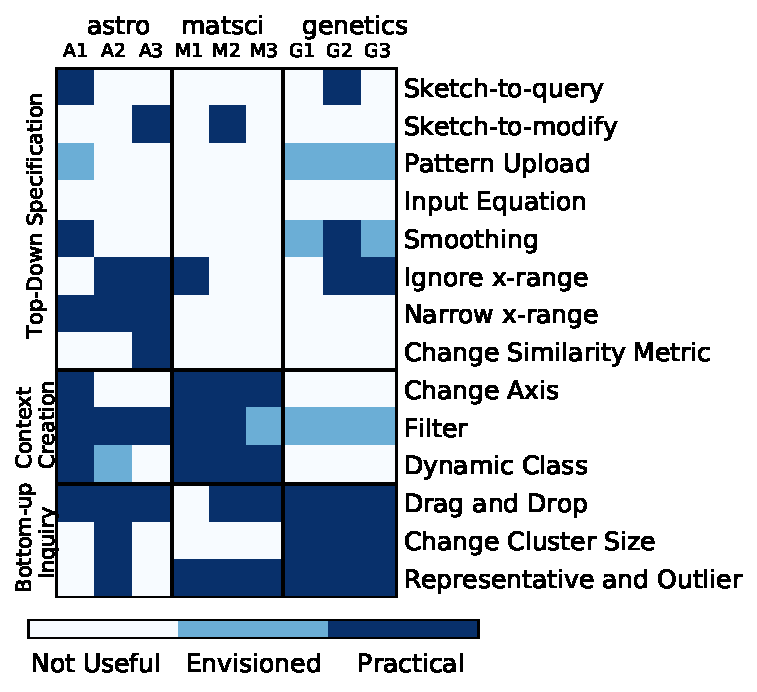
\includegraphics[width=0.8\linewidth]{figures/PENcoding.pdf}
 %   \caption{Heatmap of features categorized as practical usage (P), envisioned usage (E), and not useful (N).  \techreport{We find that participants preferred to query using bottom-up methods such as drag-and-drop over top-down approaches such as sketching or input equations. Participants found that data faceting via filter constraints and dynamic class creation were powerful ways to compare between subgroups or filtered subsets. The columns are arranged in the order of subject areas and the features are arranged in the order of the three foraging acts.}}\label{fig:feature_heatmap}
 % \endminipage
 % \end{figure*}
 Based on audio, video screen capture,
 and click-stream logs recorded
 during our \change{Phase II} evaluation study,
 we performed thematic analysis via open coding to label every event with a descriptive code. Event codes included specific feature usage,
 insights,
 provoked actions, confusion,
 need for capabilities unaddressed
 by the system, and use of external tools \achange{(see Appendix~\ref{apdx:studydetails} for details on our coding protocol)}. To characterize the usefulness
 of each feature, we further labeled whether each
 feature was useful to a particular participant's analysis.
 A feature was deemed \textit{useful}
 if the feature was either used in a sensible
 and meaningful way \change{to accomplish a task or address a question} during the study,
 or has envisioned usage outside of the constrained
 time limit during the study
 (e.g., if data was available or downstream analysis was conducted).
 We derived these labels from the study transcript
 to circumvent self-reporting bias~\cite{Williams2017},
 which can often artificially inflate
 the usefulness of the feature under examination.
 In this section, we will apply our thematic analysis results to understand how each sensemaking process occurs in practice.%real-world analytic tasks.}
 %\agp{Can't parse the previous sentence}
 %categorized the features based on whether there was a sensible usage of the feature
 % into one of the three usage types based on how each feature was used during the study:
 % \begin{denselist}
 %     \item Practical: Features used in a sensible and meaningful way.
 %     \item Envisioned: Features which could be used practically if the envisioned data was available or if they conducted downstream analysis, but was not performed due to the limited time during the study.
 %     \item Not useful: Features that are not useful or do not make sense for the participant's research question and dataset.
 % \end{denselist}
 % \par Given these initial findings, we further investigated where the `sketch'
 % Our interactions with the scientists showed that different modalities for inputting a query can be useful for different problem contexts. In addition, the three paradigms of sensemaking described earlier are not mutually exclusive. In fact, we find that participants often construct a central workflow focused on features from one of the main paradigms and interleave variations with the feature usage from the two other paradigms as they iterate on the analytic task. As shown in Figure~\ref{fig:usagefreqbysubject}, the central paradigm adopted by each use case is tightly coupled with characteristics of the analytic challenges presented by each subject area.
 % interplay
 % Next, we will describe some of the design principles (DP) based on our study findings.
 %focus on understanding the design space of VQSs and highlight the takeaways of our study.%developing a process model and design guideline for insight formation in VQSs and divert our thematic analysis of how VQSs fit into the context of an analysis workflow to our technical report.% These observation inform our ----- search-browse paradigm
 % \subsubsection{Discovery of Real-world insights}
 % \par Our participants' original workflow often required them to compare between many visualizations manually through separate analysis and visualization steps. Three of the participants cited that this segmented analyze-then-visualize workflow was one of their chief bottlenecks. The cognitive overhead from the segmented workflow made them more hesitant to visualize the results of different parameters and data operations, as A2 noted:
 % \begin{quote}
 % The quick visualization is something that I could not do on my current framework. I could not query as fast as you do; I need to wait for it, plot, and then compare. Every time I plot, I need to define subplots for 12 visualizations, then its slower. That's the reason why I sometimes plot less, and I rely more on the statistics from the likelihood tests. Sometimes I plot less than I really should be doing.
 % \end{quote}
 % The ability to rapidly experiment with large numbers of hypotheses in real time is a crucial step in the agile creative process in helping analysts discover actionable insights~\cite{Shneiderman2007a}. Five out of nine participants discussed how the dynamic, interactive update of the visualization in \zv was the main advantage for using VQSs over their original workflow.
 % \begin{figure}[h!]
 %   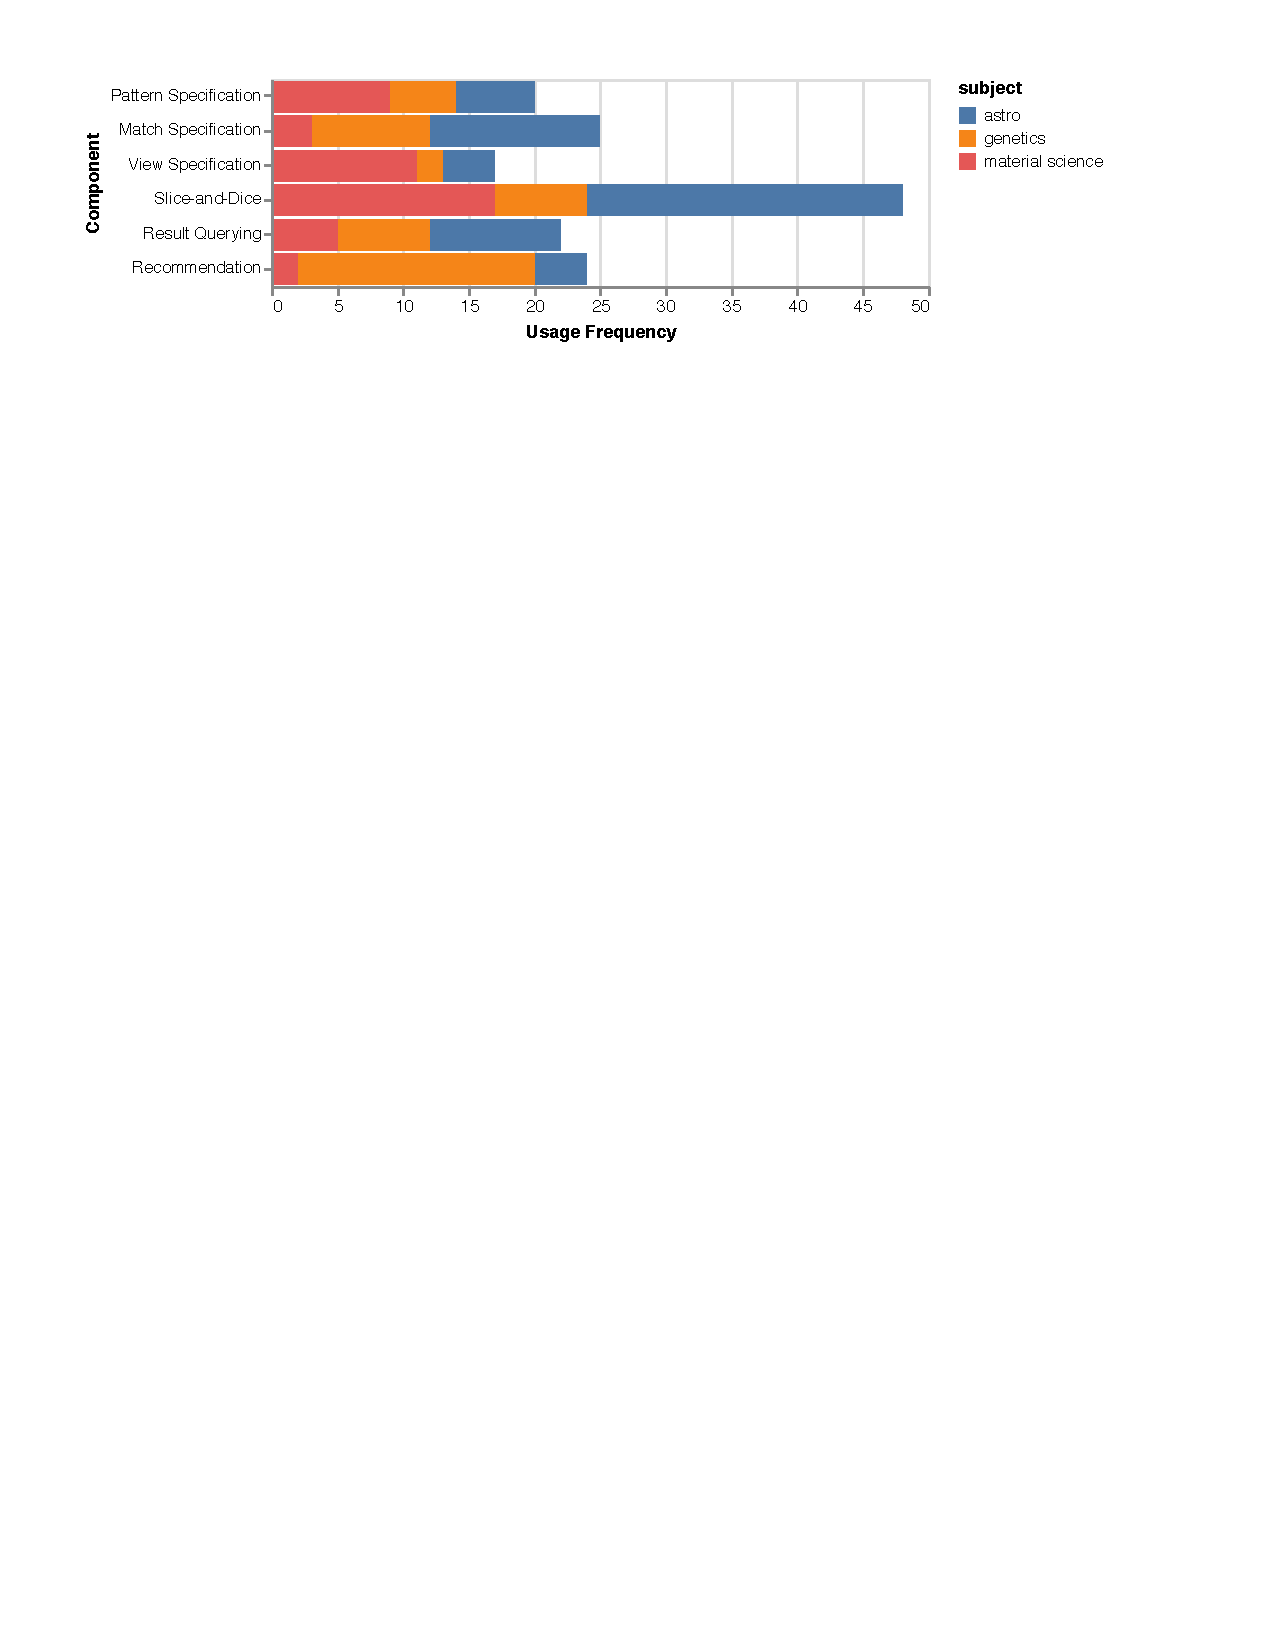
\includegraphics[width=\linewidth]{figures/usagefreqbysubject.pdf}
 %   \caption{The number of times each component is used during the evaluation study, broken down by subject areas.}\label{fig:usagefreqbysubject}
 % \end{figure}
 % \subsection{The Ineffectiveness of Sketch}
 \subsection{\change{Uncovering the Myth of Sketch-to-Insight}}
 % \subsection{DC3: Closing the loop in VQS sense-making cycle with bottom-up data-driven inquries}
 \par \change{To understand the usefulness of different visual querying modalities, we analyzed their frequency of use in our evaluation study.} To our surprise,
 despite the prevalence of sketch-to-query
 systems in the literature, \techreport{Figure \ref{fig:feature_heatmap} shows that} only two out of our nine participants
 found it useful to directly
 sketch a desired pattern onto the canvas. %Overall, bottom-up querying via drag-and-drop was more intuitive and more commonly used than top-down querying methods, such as sketching or input equations.
 The reason why most participants
 did not find direct sketching useful was that
 they often do not start their analysis with a specific pattern in mind.
 Instead, their intuition about what to query is derived
 from other visualizations they \change{encountered}
 during exploration, in which case it makes
 more sense to query using those visualizations
 as examples directly (e.g., by dragging and dropping
 that visualization onto the canvas to submit the query).
 Even if a user has a pattern in mind,
 translating that pattern into a sketch is often hard
 to do. For example,
 A2 wanted to search for a highly-varying signal
 enveloped by a sinusoidal pattern indicating
 planetary rotation 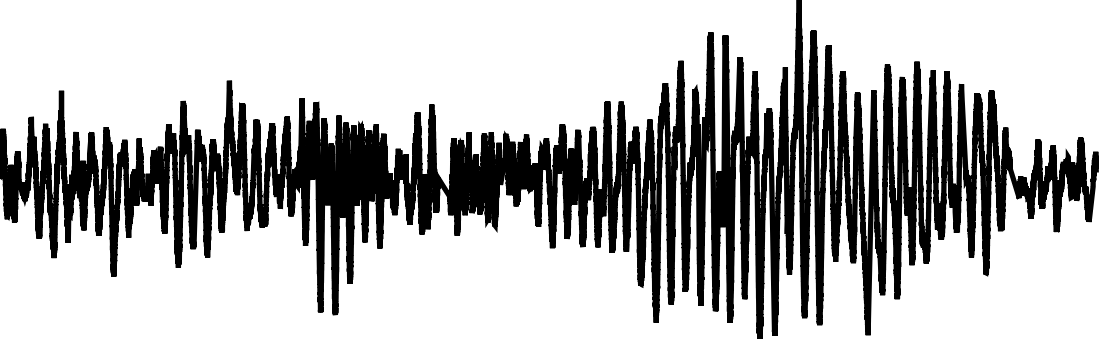
\includegraphics[width=2\baselineskip,keepaspectratio]{figures/impossible_sketch.png}, which \achange{was} hard to draw by hand.
 \begin{figure}[h!]
   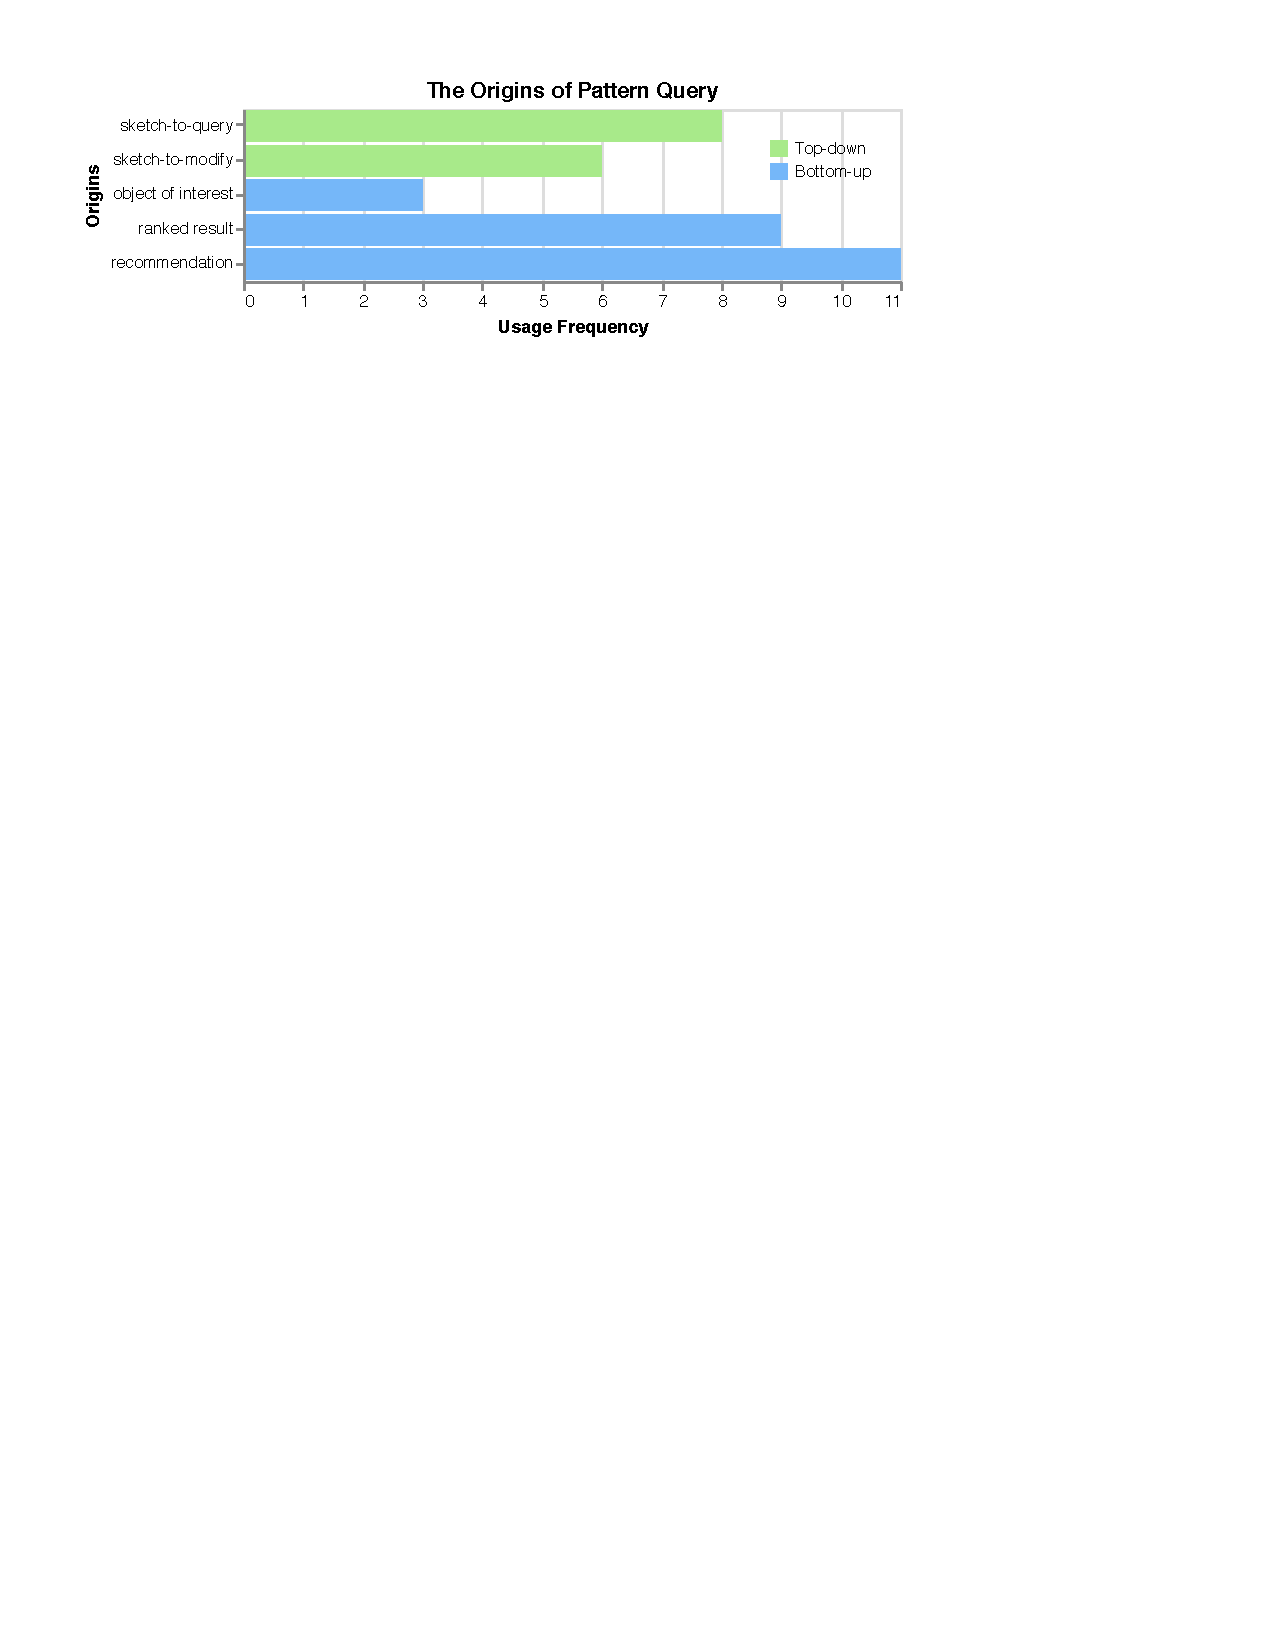
\includegraphics[width=0.95\linewidth]{figures/the_origins_of_sketch.pdf}
   \vspace{-5pt}
   \caption{The number of times a pattern query originates from one of the workflows. We find that pattern queries are far more commonly generated via bottom-up than top-down processes.}\label{fig:origins_of_sketch}
   \vspace{-5pt}
 \end{figure}
 %where the pattern on the canvas typically originates
 \par Given these initial findings,
 we further investigated \achange{the processes that participants engaged in to} construct pattern queries, as presented in Figure~\ref{fig:origins_of_sketch}.
 Pattern queries can be generated by
 either top-down (sketching) or
 bottom-up (drag-and-drop) processes,
 driven by various different querying intentions.
 Within top-down processes,
 a pattern query could arise
 from users directly sketching
 a new pattern (sketch-to-query)
 or by modifying an existing sketch (sketch-to-modify). For example, M2 first sketched a pattern
 to find solvent classes with anticorrelated
 properties without much success in returning a desired match.
 %However, the sketched query did not return visualizations of interest.
 So he instead dragged and dropped one
 of the peripheral visualizations similar
 to his desired visualization and then smoothed
 out the noise in the visualization via sketching yielding
 a straight line,
 as shown in Figure \ref{query_modification} (left).
 M2 repeated this workflow twice in separate
 occurrences during the study and
 was able to derive insights from the results.
 Likewise, Figure~\ref{query_modification} (right)
 illustrates how A3 first picked out a regular pattern
 (suspected starspot), then modified it slightly
 so that the pattern looks more irregular (to find pulsating stars).
 %Within these actions, there can be different intentions behind the sketch. While all visualizations that could be drag-and-dropped must come from the result or recommendation pane, a query can come from a particular object that the participant is interested in or simply through peripheral browsing of visualization results.%, described in the next section.
 %\par The latter case is also supported by the
 %\par There are also many unexpected use cases where sketching was simply used as a mechanism to modify an existing pattern query.
 %Likewise, A3 was interested in pulsating stars that looked similar to stellar hotspots in terms of its dramatic amplitude fluctuations, but differ in that their patterns exhibited irregularities. Figure \ref{query_modification} (right) showed how she first picked out a regular pattern (suspected star spot), then modified it slightly so that the pattern looks more irregular.
 %Likewise, A3 was interested in pulsating stars characterized by dramatic changes in the amplitudes of the light curves. During the search, hotspots on stellar surfaces often show up as false positives as they also result in dramatic amplitude fluctuations, but happen at a regular intervals. In the VQS, A3 looked for patterns that exhibits amplitude variations, but also some irregularities. As shown in Figure \ref{query_modification} (right), she first picked out a regular pattern (suspected star spot), then modified it slightly so that the pattern looks more irregular.\par While all visualizations that could be drag-and-dropped must come from the result or recommendation pane, a query can come from a particular object that the participant is interested in or simply through peripheral browsing of visualization results.
 As described in the following section,
 bottom-up pattern queries can come from either
 the ranked list of results,
 recommendations, or by selecting a
 particular object of interest as a drag-and-drop query.
 Figure~\ref{fig:origins_of_sketch} shows that
 \emph{bottom-up processes are more common
 than top-down processes for generating a pattern query}.
 \begin{figure}[h!]
     \centering
     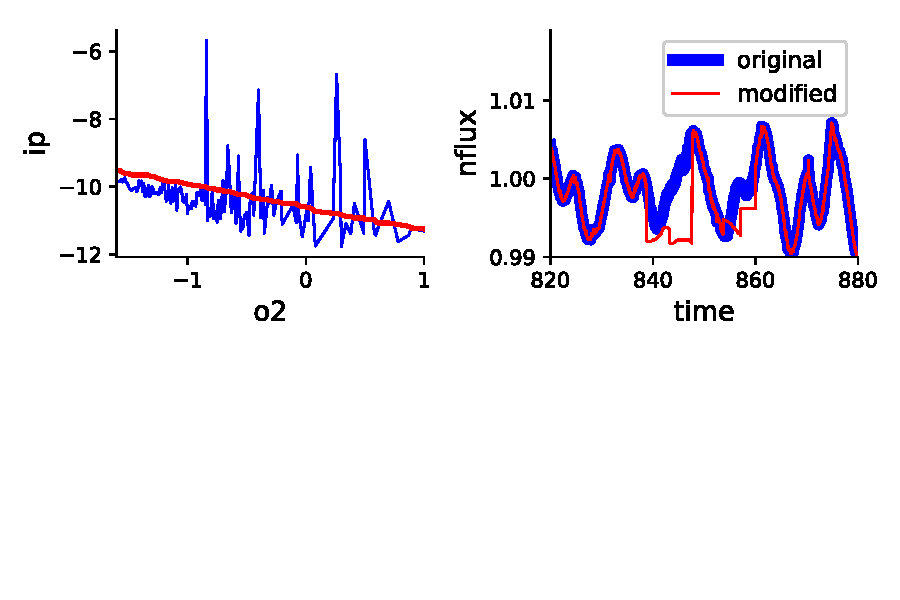
\includegraphics[width=\columnwidth]{figures/QueryModificationBySketch.pdf}
     \caption{Example of sketch-to-modify, based on canvas traces from M2 (left) and A3 (right). The original drag-and-dropped query is shown in blue and sketch-modified queries in red.}%during the study demonstrating query modification
     \label{query_modification}
     \vspace{-10pt}
 \end{figure}
 \par The lack of practical use \achange{for top-down pattern
 specification was} also reflected in the fact
 that none of the participants queried using an equation.
 In both astronomy and genetics, the visualization patterns
 resulting from complex physical processes
 that could not be written down as an equation analytically.
 Even in the case of material science when analytical
 relationships do exist, it is challenging to formulate patterns as functional forms in a prescriptive manner.
 % Despite functional fitting being common in scientific data analysis, Figure \ref{feature_heatmap} shows that
 % . However,
 \par Our findings suggest that while sketching
 is a useful construct for people to express their queries,
 \emph{the existing ad-hoc, sketch-only model for VQSs
 is insufficient \change{on its own}} without data examples
 that can help analysts jumpstart their exploration.
 In fact, from Figure~\ref{fig:origins_of_sketch},
 we can see that sketch-to-query was only used
 8 times, while the remaining querying modalities were used 29 times altogether,
 more than three times as much as sketch-to-query.
 This finding has profound implications
 on the design of future VQSs, since Table~\ref{table:relatedwork}
 suggests that past work has primarily focused
 on optimizing top-down process components,
 without considering how useful these features
 are in real-world analytic tasks.
 %missing out largely on the key components in the other two paradigms \cut{(indicated by the absence of green features on the right hand side of the table).
 We suspect that these limitations
 may be why existing VQSs are not commonly adopted in practice. \change{Note that we are not advocating for removing the \achange{natural and intuitive} sketch capabilities from future VQSs completely, but instead focusing future research and design efforts to examine other (often underexplored) VQS sensemaking processes. \achange{Such processes could be applied} in conjunction with sketching to help analysts more flexibly express their analytical goals, described next.}

 %This result points to a need for ----- in future VQSs. %This, however, points to an exciting direction for sketching interface in VQSs for developing advanced drawing and modification tools that enable more precise visualization query specification.} %ed coverage in addressing different types of analytics use cases
 %For instance, material science discovered a known inverse relationship during e xploration
 %Which is really interesting. Which is something that we observed experimentally also. That is an interesting insight right htere. This seems to suggest that there is a fundamental issue in if you want to try to get better on this axis, and get as low as possible, you lose out on the other axis.
 %once they see it they know it but they don't know beforehand
 
 \subsection{\change{Insights via Context Creation and Bottom-up Approaches}}%Approaches}
 % \dor{Might need to come up with a more descriptive name for this subsection}
 \par As alluded to earlier,
 \emph{bottom-up data-driven inquiries
 and context creation are far more commonly
 used than top-down pattern search
 when users have no desired patterns in mind},
 which is typically the case for exploratory data analysis.
 In particular, top-down approaches were only useful for 29\% of the use cases,
 whereas \change{they were} useful for 70\% of the use cases
 for bottom-up approaches and 67\%
 for context creation\footnote{See Appendix~\ref{apdx:studydetails} for details on how this measure was computed.}. We now highlight some exemplary workflows demonstrating the efficacy of the latter two sensemaking processes.
 %number of features labeled as useful divided by the product of total number of features and total number of users}
 %%The prevalence of bottom-up approaches not only point to the need for result querying, but also providing recommendations for users without desired patterns in mind.
 \par As shown in Figure~\ref{fig:origins_of_sketch},
 the most common use of bottom-up querying
 is via recommended visualizations. For example, G2 and G3 identified that
 the three representative patterns
 recommended in \zvpp corresponded
 to the same three groups of genes discussed
 in a recent publication~\cite{Gloss2017}:
 induced genes (profiles with expression levels going up 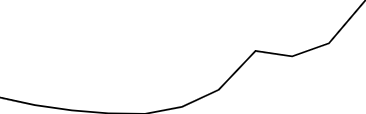
\includegraphics[width=2\baselineskip,keepaspectratio]{figures/induced.png}),
 repressed genes (starting high then decreasing 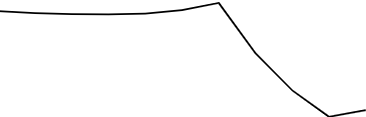
\includegraphics[width=2\baselineskip,keepaspectratio]{figures/repressed.png}),
 and transients (rising first then dropping at another time point 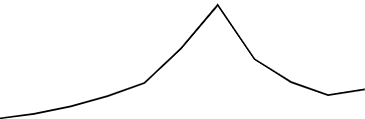
\includegraphics[width=2\baselineskip,keepaspectratio]{figures/transient.png}). The clusters provoked G2 to generate a hypothesis
 regarding the properties of transients:
 \textit{``Is that because all the transient groups
 get clustered together, or can I get sharp patterns
 that rise and ebb at different time points?''}
 To verify this hypothesis, G2 increased the parameter controlling the number of clusters and noticed that the clusters
 no longer exhibited the clean,
 intuitive patterns he had seen earlier.
 G3 expressed a similar sentiment and proceeded
 by inspecting the visualizations
 in the cluster via drag-and-drop.
 He found a group of genes that all transitioned
 at the same timestep, while others transitioned
 at different timesteps.
 \techreport{G3 described the process of using
 VQSs as doing ``detective work'' that provoked
 him to generate further scientific hypotheses
 as well as data actions.}
 \par By browsing through the ranked list of
 results in \zvpp, participants were also able to
 gain a peripheral overview of the data
 and spot anomalies during exploration.
 For example, A1 spotted time series
 that were too faint to look like stars
 after applying the filter CLASS\_STAR=1,
 which led him to discover that all stars
 have been mislabeled with CLASS\_STAR=0 as 1 during data cleaning.
 %This includes inspecting the top-most similar visualizations that lie in the queried cluster. and finding visualizations that are similar to an object of interest that exhibits a desired pattern. %. After browsing through a series query results and checking with an external database, he concluded that
  %We found that geneticists often gain their intuition about the data from the recommended representative trends. One example of rapid insight discovery
 %the dataset had been incorrectly labelled with all the stars with CLASS\_STAR=0 as 1 during data cleaning.
 %Examples of how recommended trends can provoke further insightful actions comes from G2 and G3, who identified that the three representative patterns shown in \zvpp---induced genes (profiles with expression levels staying up), repressed genes (started high but went down), and transients (go up and then come down at different time points)---corresponded to the same three groups of genes discussed in a recent publication~\cite{Gloss2017}.
 % \subsection{Enriching Search with Context}
 \begin{figure*}[ht!]
   \centering
   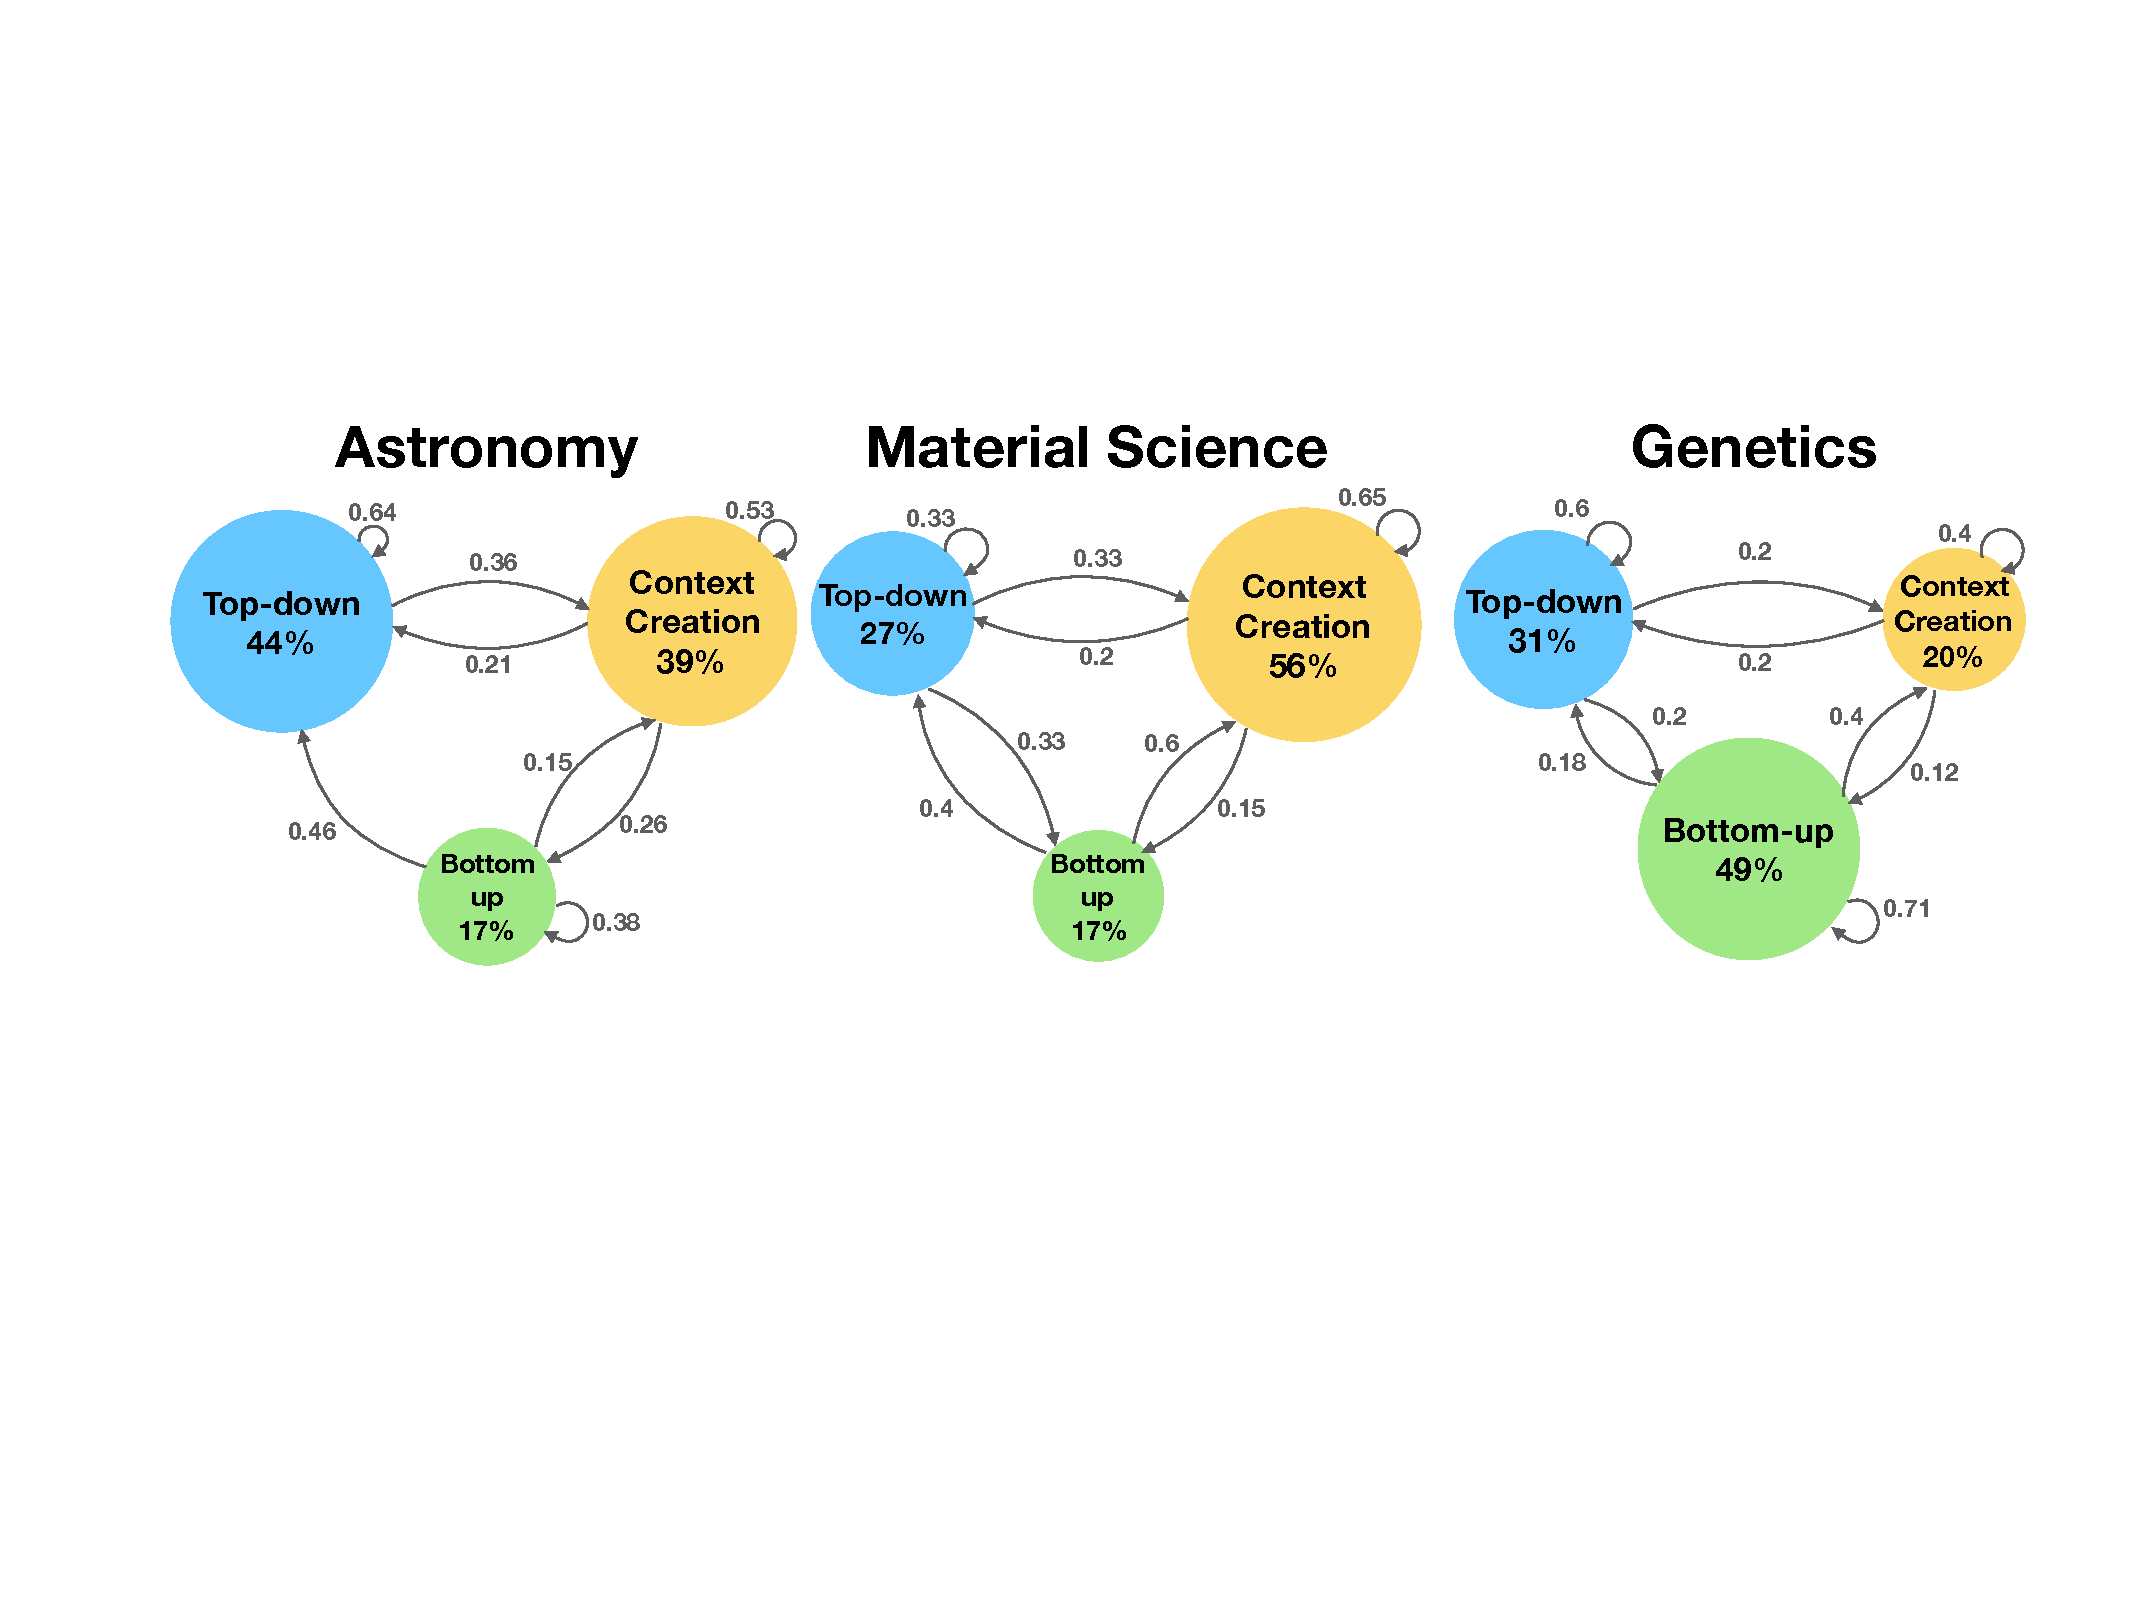
\includegraphics[width=0.6\linewidth]{figures/markov_transition.pdf}
   \caption{Markov models computed based on evaluation study event sequences, with edges denoting the probability that participant in the particular domain will go from one sensemaking process to the next. Nodes are scaled according to \change{their} eigenvector centrality, representing the percentage of time participants would spend in a particular sensemaking process in steady state. \achange{Markov models are computed based on a total of 206 event actions taken by participants during the evaluation study (80 for astronomy, 65 for genetics, and 61 for material science).}}\label{fig:transition}
   \vspace*{-15pt}
 \end{figure*}
 \par Past studies in visual analytics
 have shown that it is important to design features
 that enable users to select relevant subsets of data~\cite{Amar2005,Heer2012}.
 Context creation in VQSs enables users to change the ``lens''
 by which they look through the data
 when performing visual querying,
 thereby creating more opportunities
 to explore the data from different perspectives. All participants found at least
 one of the features in context creation to be useful.
 %We designed two dynamic faceting features coupled with coordinated views that enabled users to specify subsets of data they are querying on and see immediate changes updated in the query, representative, and outlier results.
 %either envisioned a use case or utilized features in the context creation paradigm to explore and compare subsets of their data.
 %ven though the filtering step could be easily done with an external tool and reloaded into \zv, filtering on-the-fly was a powerful way to dynamically test his hypothesis. I
 \par Both A1 and A2 expressed that context creation through interactive filtering enabled them to test conditions and tune values that they would not have otherwise modified, effectively lowering the barrier between the iterative hypothesize-then-compare cycle during sensemaking.
 % echoing our previous finding that segmented workflow prevents extensive exploration.
 During the study, participants used filtering
 to address questions such as:
 \textit{Are there more genes similar
 to a known activator when we subselect
 only the differentially expressed genes?} \techreport{\texttt{DIFFEXP=1} }(G2) or \textit{Can I find more supernovae candidates if I query only on objects that are bright and classified as a star?} \techreport{\texttt{flux\textgreater10 AND CLASS\_STAR=1} }(A1). Three participants had also used filtering as a way to query with known individual objects of interest, as shown in Figure~\ref{fig:origins_of_sketch}. For example, G2 set the filter as gene=9687 and explained that since ``\textit{this gene is regulated by the estrogen receptor, when we search for other genes that resemble this gene, we can find other genes that are potentially affected by the same factors.}''
 \par While filtering enabled users to
 narrow down to a selected data subset,
 dynamic classes (buckets of data points that satisfies one or more range constraints) enabled users to compare
 relationships between multiple attributes and subgroups of data.
 For example, M2 divided solvents in the database
 into eight different categories based on voltage properties,
 state of matter, and viscosity levels,
 by dynamically setting the cutoff values
 on the quantitative variables to create these classes.
 By exploring these custom classes, M2 discovered that the relationship between viscosity and lithium solvation energy is independent of whether a solvent belongs to the class of high voltage or low voltage solvents. He cited that dynamic class creation was central to learning about this previously-unknown attribute properties:
 \begin{quote}
 All this is really possible because of dynamic class creation, so this allows you to bucket your intuition and put that together. [...] I can now bucket things as high voltage stable, liquid stable, viscous, or not viscous and start doing this classification quickly and start to explore trends. [...] look how quickly we can do it!% Quite good!
 \end{quote}
 %Context creation is a useful ---- despite the --- pattern instance. Filtering still useful
 %\par Participants employed \emph{a mix of bottom-up and top-down approaches when faceting through data in VQS}, including narrowing the search space based on some intuition about a phenomena, selecting individual visualizations, or specifying high-level groupings to compare and query with.
 \subsection{Combining Sensemaking Processes in VQS Workflows}
 Given our observations so far as to  how participants make use of each sensemaking process in practice, we further investigate the interplay between these sensemaking processes in the context of an analysis workflow. %interplay with each other dynamically i% - Bottom up and context creation much more common than top-down. Stats \%. Brief Examples of each (How they are used in practice).
 % - BUT All three process are equally important.
 % - participants can go from one to the next and there is no single progression (e.g. context --> bottom -up --> top-down).
 % - Both the PageRank score (how important/“central” is the state is to the analysis?), raw occurrence of each state (how frequently is a feature categorized as part of the state used?) and the normalized self-directed edge score (how much user stays in that state?) coincide with what each subject area focuses on.
 % We first examine the popularity of each sensemaking process based on how frequently they are used in the study. Figure~\ref{fig:feature_heatmap} show that features categorized as bottom-up (useful for 70\% of the use cases) and context creation (67\%) are much more useful compared top-down features (29\%). [Examples of Bottom up]. [Examples of Context Creation].
 %Despite differing in levels of usage, each sensemaking process fulfills a central role in participants' analysis.
 % illustrates the state transitions computed based on event sequences from the evaluation study. %stay in the same state.
 %Figure~\ref{fig:taxonomy},
 The event sequences from the evaluation study
 consist of labels describing when specific features were used.
 Using the taxonomy in Table~\ref{bigfeaturetable}, we map each usage of a feature in \zvpp to one of the three sensemaking processes.
 Each participant's event sequence
 is divided into sessions,
 each indicating a separate line of inquiry
 during the analysis.
 Based on these event sequences---one for each session,
 we compute the aggregate state transition probabilities
 (edge weight labels in Figure~\ref{fig:transition})
 to characterize how participants from each domain
 move between different sensemaking processes.
 For example, in material science,
 bottom-up exploration
 leads to context creation 60\% of the time
 and to top-down pattern search
 the rest of the time.
 Self-directed edges indicate the probability that the participant
 would continue with the same type of sensemaking process.
 For example, when an astronomer performs top-down pattern search,
 it is followed by another top-down process 64\% of the time and context creation the rest of the time,
 but never followed by \change{a bottom-up process}.
 This high self-directed transition probability
 reflects how astronomers often need to iteratively
 refine their top-down query through pattern
 or match specification when looking for a specific pattern. %when A1 looks for supernovae, he needs to iteratively refine his top-down query through pattern or match specification interfaces. %He could also chose to refine ----- , control --- to issue the desired query.
 %Each event sequence is separated by labeled session breaks signaling the beginning of a new line of inquiry. The
 % \begin{figure}[ht!]
 %   \centering
 %   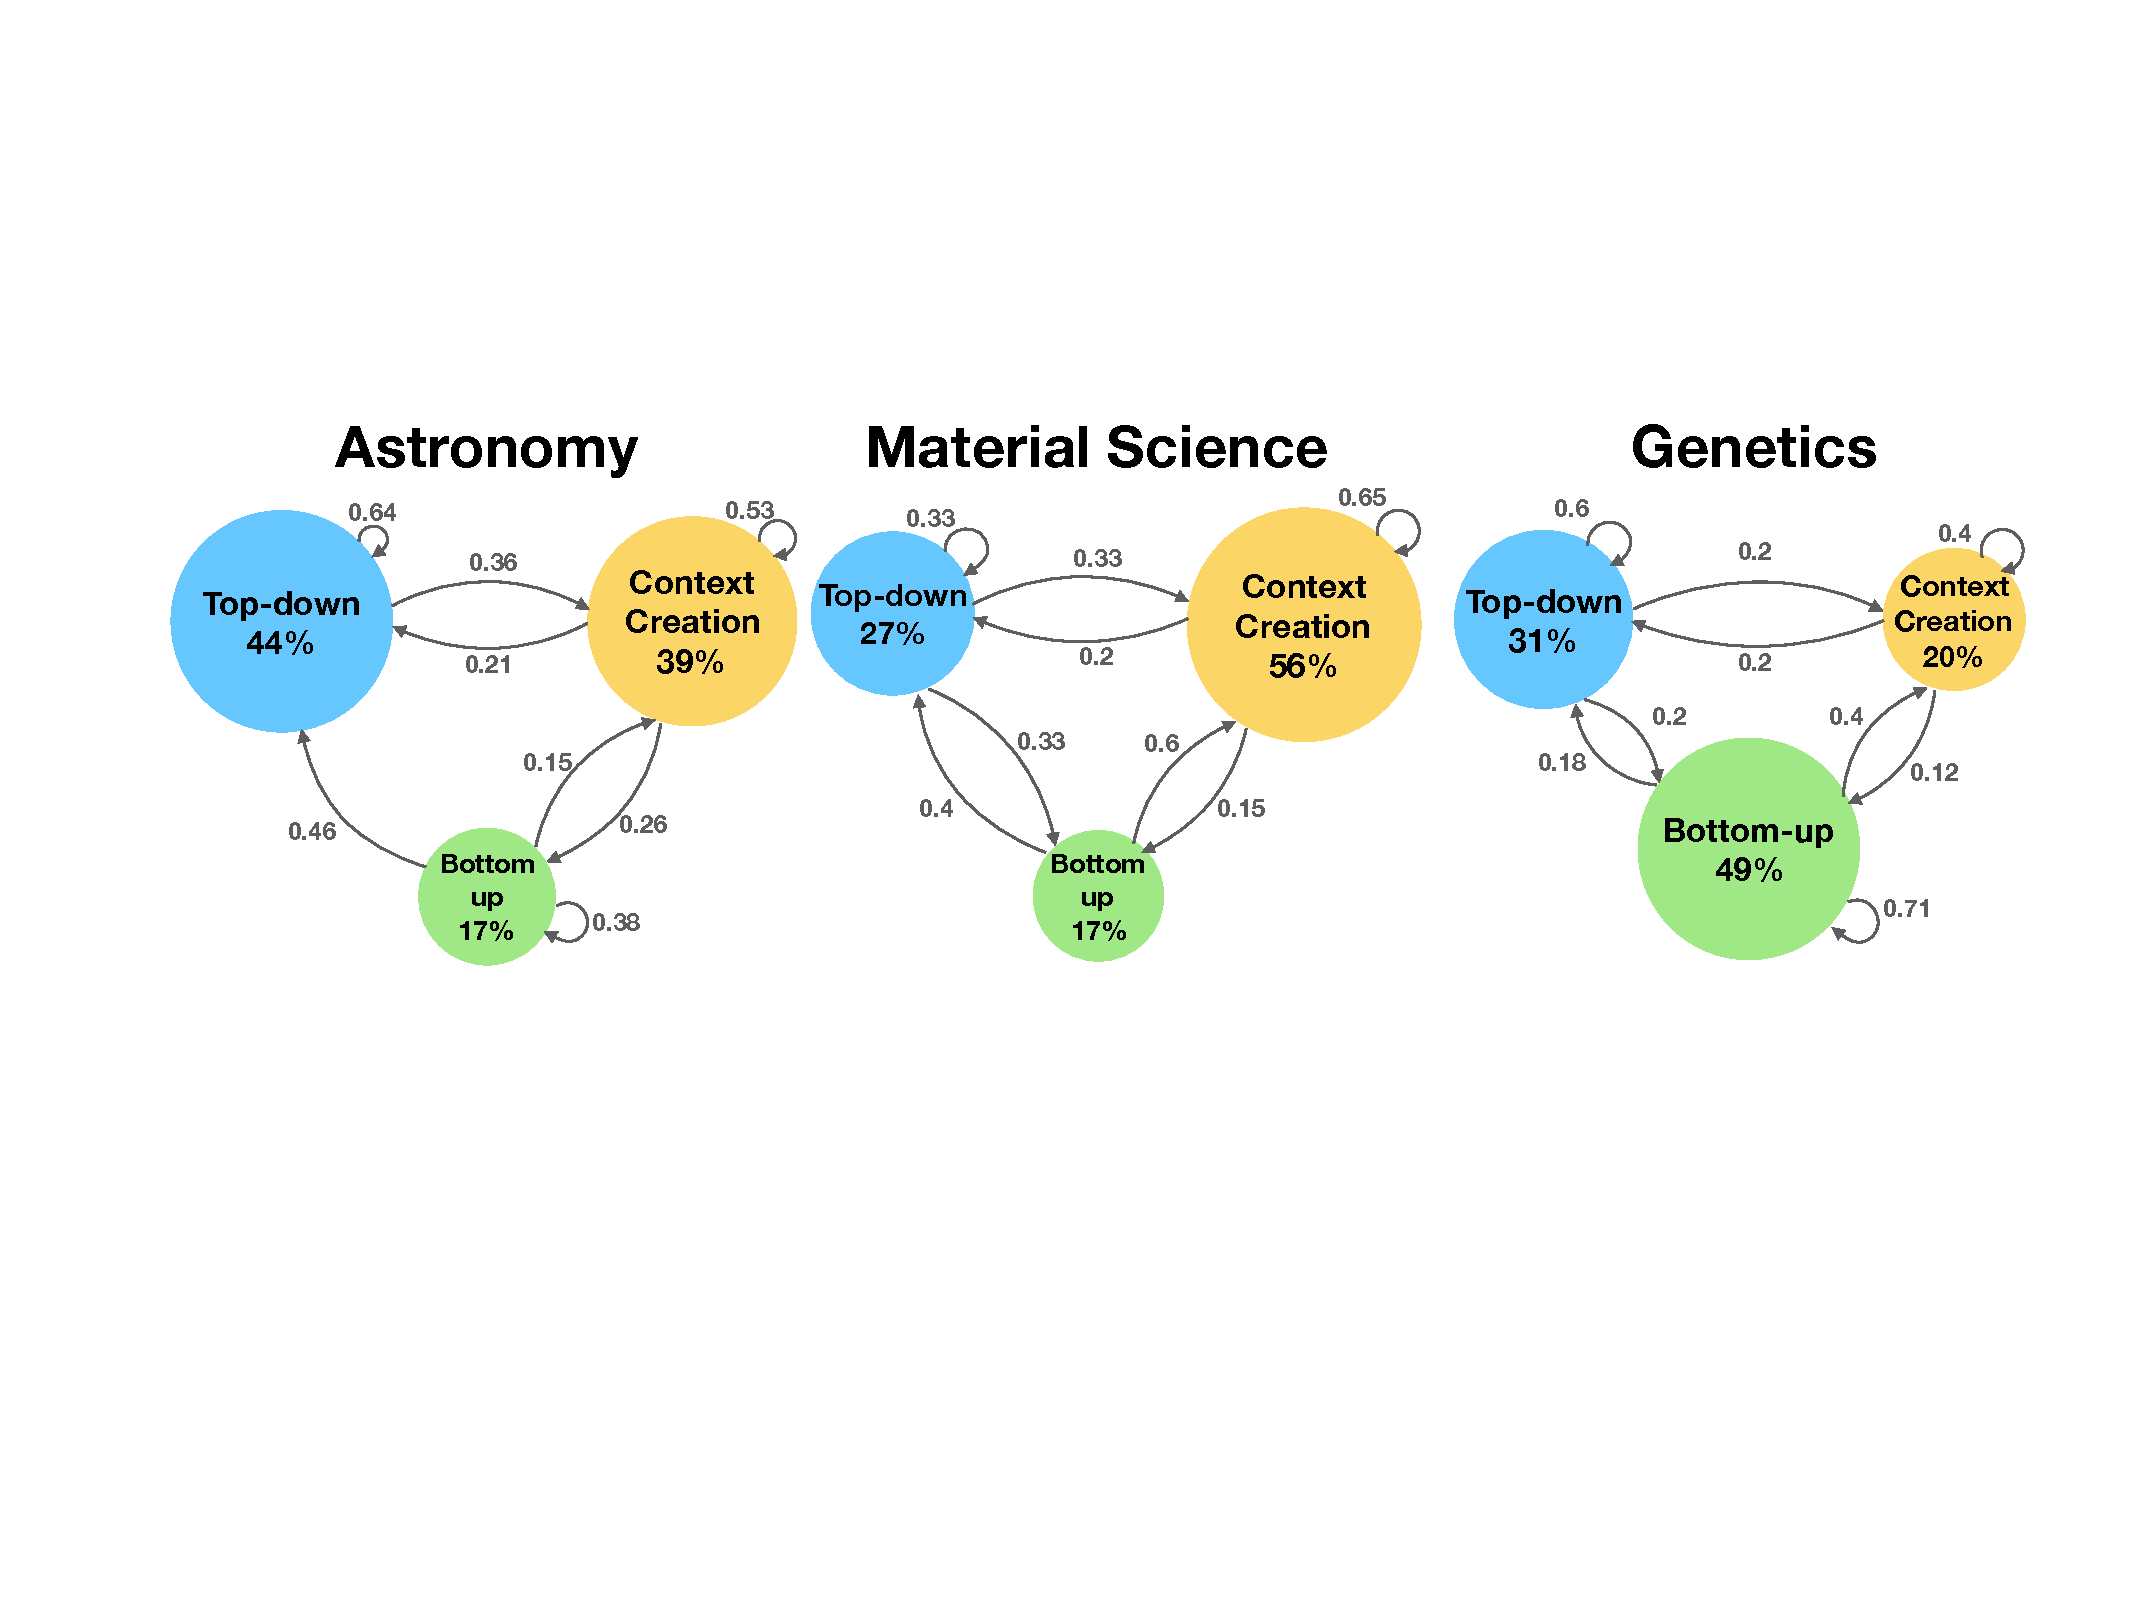
\includegraphics[width=\linewidth]{figures/markov_transition.pdf}
 %   \caption{Markov models computed based on evaluation study event sequences, with edges denoting the probability that participant in the particular domain will go from one sensemaking process to the next. Nodes are scaled according to the eigenvector centrality, representing the percentage of time participants would spend in a particular sensemaking process in steady state.\label{fig:transition
 %   \vspace*{-5pt}
 % \end{figure}
 % Similar to the sensemaking model proposed by Pirolli and Card~\cite{Pirolli}, the ---- sensemaking loop representing iterative process
 % ---- highlights how the two newly discovered VQS sensemaking process in this paper are essential for `closing the loop' between the sensemaking acts in VQSs. %, equally important
 % both the browsing-act through recommendations and performing search via these results are
 %These examples show that both the browsing-act through recommendations and performing search via these results are
 %The three sensemaking ----- not mutually exclusive, participants can go from one to the next and there is no single progression (e.g. context --> bottom -up --> top-down). Iterative blah blah. three process are equally important.
 %The three paradigms of sensemaking described earlier are not mutually exclusive.
 %Different sensemaking processes can be useful for different problem contexts.
 \par To study how important each sensemaking process
 is for participant's overall analysis,
 we compute the eigenvector centrality of each graph,
 displayed as node labels in Figure~\ref{fig:transition}.
 These values represent the percentage of time the participants
 spend in each of the sensemaking processes
 when the transition model has evolved to a steady state~\cite{pierre2011}.
 Given that nodes in Figure~\ref{fig:transition}
 are scaled by this value, in all domains,
 we observe that there is always a prominent node
 connected to two less prominent ones---but it is also clear
 that all three nodes are essential to all domains.
 Our observation demonstrates how \emph{participants
 often construct a central workflow
 around a main sensemaking process \change{based on their analytical \textbf{goals}
 and interleave variations with the two other \textbf{support} processes as they iterate on the analytic task}}, as illustrated in Table~\ref{science_task}. For example, \change{the} material scientists focus on context creation 56\% of the time, mainly through dynamic class creation,
 followed by bottom-up inquiries (such as drag-and-drop)
  and top-down pattern searches (such as sketch modification).
 %through dynamic classes than top-down pattern search. %astronomers focus largely on performing top-down pattern search, while filtering on the visualization space. %in Section~\ref{sec:pd_findings}}.
 The central process adopted by each domain
 is tightly coupled with the problem characteristics associated with each domain. For example, without an initial query in mind,
 geneticists relied heavily on bottom-up querying
 through recommendations to jumpstart their queries.
 %Despite the differing levels of usage from each subject area, we learn that \textit{each sensemaking process fulfills a central role in participants' analysis to address their high-level research objectives}.
 % \agp{maybe point to figure?}.
 % they brought to the study
 %pattern instance and visualized attributes
 \par The Markov transition model exemplifies how participants
 adopted a diverse set of workflows
 based on their unique set of research questions. The bi-directional and cyclical nature
 of the transition graphs in Figure~\ref{fig:transition} highlight how the three sensemaking processes do not simply follow a linear progression towards finding a single pattern or attribute of interest. %, going from unknown to known in the Figure~\ref{2dmodel problem space}
 Instead, the high connectivity of the transition model illustrates how these three equally-important processes form a sensemaking loop, representing iterative acts of dynamic foraging and hypothesis generation. \change{This finding reinforces the importance of each sensemaking process and indicates that future VQSs need to be \emph{integrative} in supporting all three sensemaking process to enable a diverse set of potential workflows for addressing a wide range of analytical inquiries.} %This flexibility is enabled by the diverse set of potential workflows that could be constructed in an integrative VQS like \zvpp, for addressing a wide range of analytical inquiries.%single-directional%. The VQS sensemaking loop%full-fledged
 \subsection{Limitations}%suggests that direct sketch is inefficient
 \par Although evidence from our evaluation study \change{points to the infrequent use of direct sketch}, we have not performed controlled studies with a sketch-only system as a baseline to validate this hypothesis. The goal of our study is to uncover qualitative insights that might reveal why VQSs are not widely used in practice; further validation of specific findings is out of the scope of this paper. \change{While concerns regarding study results being focused on \zvpp must be acknowledged, we note that \zvpp is one of the most comprehensive VQSs to-date, covering many of the features from past systems and more (as evident from Table 1). We believe that our integrative VQS, \zvpp, can serve as a baseline for future research in VQS to evaluate against and build upon.} Given that this paper covered three design studies along with one evaluation study, we were unable to cover each domain to the level of detail typically found in a dedicated design study paper. Instead, our focus was to highlight the differences and similarities among these domains relevant to the capabilities required in VQS and we defer domain-specific participatory design details and artifacts to Appendix~\ref{apdx:pdartifact}. \achange{Future longitudinal studies may also help alleviate the novelty effects that participants may have experienced during the evaluation study.} While we have generalized our findings \change{beyond existing work} by employing three different and diverse domains (see Figure~\ref{fig:transition}),
 our case studies have so far
 been focused on scientific data analysis \change{with domain-experts},
 as a first step towards greater adoption of VQSs.
 Other potential domains that could benefit from VQSs include:
 financial data for business intelligence,
 electronic medical records for healthcare,
 and personal data for ``Quantified Self''.
 These different domains may each pose different sets of challenges \change{(such as designing for novices as end-users)} unaddressed by the findings in this paper,
  pointing to a promising direction for future work.